\documentclass[conference]{IEEEtran}
\IEEEoverridecommandlockouts

\usepackage{cite}
\usepackage{amsmath,amssymb,amsfonts}
\usepackage{algorithmic}
\usepackage{graphicx}
\usepackage{textcomp}
\usepackage{xcolor}
\usepackage{booktabs}
\usepackage{multirow}
\usepackage{url}
\usepackage{listings}
\usepackage{tikz}
\usetikzlibrary{shapes.geometric, arrows, positioning}

%% Fill every \RESULT{} before submission -- never submit with red placeholders
\newcommand{\RESULT}[1]{\textbf{\textcolor{red}{[FILL: #1]}}}

\def\BibTeX{{\rm B\kern-.05em{\sc i\kern-.025em b}\kern-.08em
    T\kern-.1667em\lower.7ex\hbox{E}\kern-.125emX}}

\begin{document}

\title{Pre-Synthesis Safety Auditing of Industrial Control\\
Specifications Using a Neuro-Symbolic Framework}

\author{
  \IEEEauthorblockN{Lokani Rakesh}
  \IEEEauthorblockA{
    \textit{Department of Computer Science \& Engineering}\\
    \textit{Amrita Vishwa Vidyapeetham}\\
    Coimbatore, India\\
    \texttt{[YOUR EMAIL]@students.amrita.edu}
  }
  \and
  \IEEEauthorblockN{Dr. Raviteja [SURNAME]}
  \IEEEauthorblockA{
    \textit{Department of Computer Science \& Engineering}\\
    \textit{Amrita Vishwa Vidyapeetham}\\
    Coimbatore, India\\
    \texttt{[GUIDE EMAIL]@amrita.edu}
  }
}

\maketitle

\begin{abstract}
Safety-critical industrial control systems are programmed from engineering
specification documents---control narratives, cause-and-effect tables, and
P\&ID diagrams---that are authored informally, without machine-checkable
structure. AI-assisted PLC code generation tools translate these documents
into executable logic, but none of them check whether the source specification
is internally consistent or complete. A specification missing a high-pressure
shutdown rule will be faithfully translated into PLC code that also lacks the
shutdown rule; no post-generation verification can recover a constraint that
was never written.

We address this gap by auditing specifications \emph{before} PLC code is
generated. Our framework extracts entities and control rules from multimodal
specification documents using a locally-deployed LLM (Qwen~2.5), links
extracted entities across document modalities using a three-step cascade
(exact match, fuzzy Levenshtein, sentence-transformer embedding), and
formally verifies the extracted rule set against a library of 16
IEC~61511/ISA-84 aligned safety invariants using the Z3 SMT solver.
The neural and symbolic components are architecturally separated: the LLM
performs only extraction; all safety reasoning is delegated to Z3.

On a synthetic benchmark of 50 annotated specification packages
with injected defects, the framework achieves overall precision~0.615,
recall~0.800, and F1-score~0.696. Omission-type defects---the class
structurally undetectable by post-generation verification---achieve
recall~1.000 for both missing-shutdown-rule and missing-alarm categories,
directly validating the pre-synthesis gap claim. Application to a
Schneider~Electric industrial control narrative is currently under
domain review; preliminary results indicate the framework generalises
to authentic industrial specifications beyond the synthetic benchmark.
\end{abstract}

\begin{IEEEkeywords}
Industrial Control Systems, Safety Auditing, Neuro-Symbolic AI, PLC,
Z3 SMT Solver, IEC 61511, Formal Verification, Large Language Models
\end{IEEEkeywords}

%% ---------------------------------------------------------------
\section{Introduction}

Programmable Logic Controllers (PLCs) govern safety-critical
industrial processes---chemical reactors, refinery separation units,
gas compressor stations, and water treatment facilities. A PLC executes
control logic compiled from engineering specification documents written
by process safety engineers: control narratives in prose, cause-and-effect
(C\&E) tables listing trip conditions, and P\&ID diagrams depicting equipment
connectivity. These documents are the \emph{ground truth} from which
control logic is derived.

Recent work on AI-assisted PLC generation translates these specifications
directly into IEC~61131-3 programs~\cite{paliwal2021digitize,koziolek2023chatgpt,
fakih2024llm4plc}. The driving motivation is reducing manual coding effort
and transcription errors. However, every approach in this space operates
under a shared and unexamined assumption: that the specification being
translated is correct. Generation fidelity is measured by how closely
the output code matches the specification, not by whether the specification
itself encodes a safe control strategy.

This assumption breaks down in practice. Industrial incident investigations
consistently identify specification-stage omissions as root causes. A
control narrative stating ``if pressure rises above alarm setpoint, alert
operator'' satisfies a syntactic description of alarm logic, yet it omits
the safety-critical shutdown condition: ``if pressure exceeds high-high
setpoint, stop pump immediately.'' A PLC code generator translating this
narrative faithfully will produce code that raises an alarm but does not
shut down the pump. No post-generation formal verification will detect the
omission, because the missing shutdown produces no code---and therefore no
constraint to check.

We call this the \emph{pre-synthesis gap}: the structural inability of
post-generation verification to detect specification-level omissions
and contradictions. Fig.~\ref{fig:workflow} illustrates the gap and
where our framework intervenes.

\begin{figure}[t]
\centering
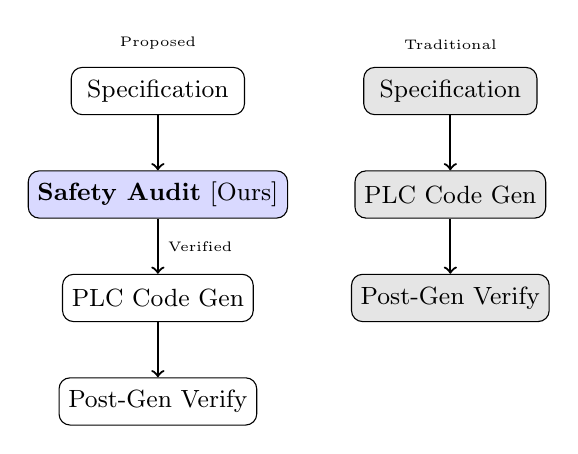
\begin{tikzpicture}[
  box/.style={rectangle, draw, rounded corners, minimum width=2.2cm,
              minimum height=0.6cm, text centered, font=\small},
  arr/.style={->, thick},
  node distance=0.7cm
]
%% Left column: proposed pipeline
\node[box] (spec) {Specification};
\node[box, below=of spec] (audit) [fill=blue!15] {\textbf{Safety Audit} [Ours]};
\node[box, below=of audit] (gen) {PLC Code Gen};
\node[box, below=of gen] (verify) {Post-Gen Verify};
\draw[arr] (spec) -- (audit);
\draw[arr] (audit) -- node[right,font=\tiny]{Verified} (gen);
\draw[arr] (gen) -- (verify);
%% Right column: traditional pipeline
\node[right=1.5cm of spec, box, fill=gray!20] (trad) {Specification};
\node[below=0.7cm of trad, box, fill=gray!20] (tgen) {PLC Code Gen};
\node[below=0.7cm of tgen, box, fill=gray!20] (tv) {Post-Gen Verify};
\draw[arr] (trad) -- (tgen);
\draw[arr] (tgen) -- (tv);
\node[font=\tiny, above=0.1cm of trad] {Traditional};
\node[font=\tiny, above=0.1cm of spec] {Proposed};
\end{tikzpicture}
\caption{Proposed pre-synthesis auditing pipeline (left) vs.\ the traditional
pipeline (right). Our safety audit intercepts specification-level defects
before PLC synthesis; post-generation verification cannot.}
\label{fig:workflow}
\end{figure}

The contributions of this work are:
\begin{enumerate}
\item A multimodal ICS specification ingestion pipeline that extracts
  structured information from control narratives, C\&E tables, and
  P\&ID diagrams as unified input, without requiring the documents to
  be reformatted or re-authored.
\item A neuro-symbolic extraction architecture in which LLM inference
  is strictly confined to entity and rule extraction---all safety
  reasoning is delegated to the Z3 SMT solver, which provides formal
  soundness guarantees~\cite{moura2008z3}.
\item A cross-modal entity linking cascade that resolves the same
  physical asset across document modalities using tag matching and
  sentence-level embedding similarity, enabling detection of cross-modal
  inconsistencies invisible to single-document analysis.
\item A formally-grounded safety invariant library of 16 templates
  aligned to IEC~61511-1 clause-level requirements, serving as the
  specification oracle for omission and contradiction detection.
\item An empirical evaluation on a 50-package annotated synthetic
  benchmark and a real Schneider Electric industrial control narrative.
\end{enumerate}

%% ---------------------------------------------------------------
\section{Related Work}

\subsection{P\&ID-to-PLC Generation}
Graph-based extraction methods parse Piping and Instrumentation
Diagrams into graph structures and derive PLC logic from topology and
connectivity~\cite{paliwal2021digitize}. Paliwal et al.\ construct
a complete automated pipeline for extracting graph-structured information
from scanned P\&ID images, demonstrating high accuracy on symbol and
connector detection. While such approaches identify equipment relationships
and loop structures directly from the diagram, they are bounded by
what the P\&ID contains. A missing safety interlock---one that the
P\&ID simply does not show---cannot be recovered by any graph traversal.
Our work processes the P\&ID as one of three input modalities and
cross-references its tag inventory against the control narrative and
C\&E table; discrepancies between modalities become findings.

\subsection{Natural Language to PLC Conversion}
LLM-based translation approaches~\cite{koziolek2023chatgpt,fakih2024llm4plc}
take prose control narratives as input and produce IEC~61131-3 Structured
Text. Koziolek et al.\ evaluate ChatGPT on industrial PLC programming
tasks, finding that while the model generates syntactically valid programs,
it lacks awareness of safety completeness requirements---a finding that
directly motivates the pre-synthesis gap framing in this work.
Fakih et al.\ extend this with formal verification of generated programs,
but note that verification can only check what is in the generated code.
Evaluation in both approaches measures \emph{translation fidelity}:
does the generated code match the intent expressed in the specification?
Fidelity-oriented evaluation does not question whether the specification
expresses a complete and safe intent. A specification that faithfully
describes an incomplete control strategy produces faithfully broken PLC
code; fidelity metrics will score this as success.

\subsection{Post-Generation Formal Verification}
SMT solvers and model checkers have been applied to verify PLC programs
after generation~\cite{mery2011event_b,clarke1999model}. These are
well-established and powerful techniques for verifying properties of
\emph{existing} code. Their structural limitation for our setting is
precise: they reason over the constraints that are present in the code.
A shutdown rule absent from the specification generates no code, and
therefore no clause for the verifier to check. The pre-synthesis gap
is opaque to post-generation verification by construction.

\subsection{HAZOP and Functional Safety Standards}
Hazard and Operability (HAZOP) analysis is the process industry's
primary method for identifying specification-level hazards~\cite{leveson2011}.
IEC~61511~\cite{iec61511} mandates HAZOP-style studies as part of Safety
Instrumented System design. HAZOP is effective: it produces a structured
examination of each process node against defined guide words. The method
is also labour-intensive---a single refinery unit HAZOP can require weeks
of structured review meetings by multiple qualified engineers. The goal of
this work is not to replace HAZOP but to provide a computational tool that
can flag candidate specification gaps \emph{before} a formal HAZOP study,
reducing engineer preparation time and providing an automated cross-check
for simpler specifications where full HAZOP may not be conducted.

\subsection{Formal Tools for Structured Specifications}
SCADE Suite~\cite{scade} and Simulink Design Verifier apply formal methods
to safety-critical specifications. Both tools operate on their own structured
modelling languages---SCADE models or Simulink diagrams---and provide strong
formal guarantees within those formats. Industrial engineering specifications
are routinely authored as free-text narratives and tabular documents;
converting these to SCADE or Simulink models requires the same manual engineering
effort as writing the PLC code. Our framework accepts the documents in their
as-authored form.

\subsection{Positioning Summary}
Table~\ref{tab:comparison} contrasts existing approaches with ours across
three dimensions: input format, whether the approach can detect missing
constraints (not just incorrect ones), and whether the analysis is automated.
To the best of our knowledge, no prior system accepts unstructured multimodal
ICS specifications as direct input and applies SMT-based formal verification
to the extracted logic before code synthesis.

\begin{table}[t]
\caption{Comparison of Related Approaches}
\label{tab:comparison}
\centering
\small
\begin{tabular}{@{}lccc@{}}
\toprule
\textbf{Approach} & \textbf{Input format} & \textbf{Detects} & \textbf{Auto-}\\
 & & \textbf{omissions?} & \textbf{mated?} \\
\midrule
P\&ID digitization~\cite{paliwal2021digitize}  & Diagram        & No          & Yes \\
NL-to-PLC~\cite{koziolek2023chatgpt}           & Narrative      & No          & Yes \\
Post-gen.\ verify.~\cite{mery2011event_b}      & PLC code       & No          & Yes \\
HAZOP~\cite{leveson2011}             & Spec.          & Yes         & No  \\
SCADE~\cite{scade}                   & SCADE model    & Yes         & Yes \\
\textbf{This work}                   & \textbf{Multi-modal spec.} & \textbf{Yes} & \textbf{Yes} \\
\bottomrule
\end{tabular}
\end{table}

%% ---------------------------------------------------------------
\section{Framework Architecture}

The framework follows a nine-phase pipeline shown in
Fig.~\ref{fig:architecture}. The architectural principle underlying the
design is a strict boundary between neural and symbolic computation,
motivated by the neuro-symbolic AI literature~\cite{garcez2019}.
LLMs are competent at extracting structured information from natural
language~\cite{qwen2024} but unreliable when asked to make safety
judgements~\cite{huang2023hallucination}. The Z3 SMT solver is sound and
complete within its decidable theories but cannot process unstructured text.
We exploit the strength of each: LLM inference handles all text
understanding; Z3 handles all safety reasoning.

\begin{figure}[t]
\centering
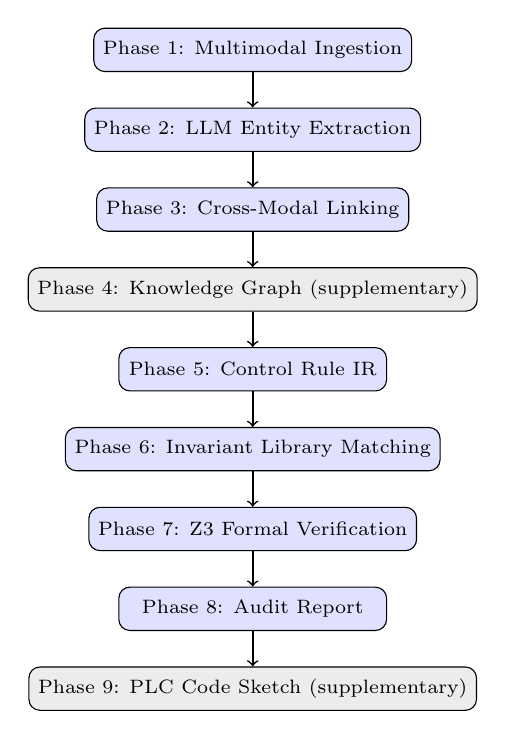
\begin{tikzpicture}[
  phase/.style={rectangle, draw, rounded corners, minimum width=3.4cm,
                minimum height=0.55cm, text centered, font=\scriptsize},
  core/.style={phase, fill=blue!12},
  supp/.style={phase, fill=gray!15},
  arr/.style={->, semithick},
  node distance=0.45cm
]
\node[core] (p1)  {Phase 1: Multimodal Ingestion};
\node[core, below=of p1] (p2)  {Phase 2: LLM Entity Extraction};
\node[core, below=of p2] (p3)  {Phase 3: Cross-Modal Linking};
\node[supp, below=of p3] (p4)  {Phase 4: Knowledge Graph (supplementary)};
\node[core, below=of p4] (p5)  {Phase 5: Control Rule IR};
\node[core, below=of p5] (p6)  {Phase 6: Invariant Library Matching};
\node[core, below=of p6] (p7)  {Phase 7: Z3 Formal Verification};
\node[core, below=of p7] (p8)  {Phase 8: Audit Report};
\node[supp, below=of p8] (p9)  {Phase 9: PLC Code Sketch (supplementary)};
\foreach \a/\b in {p1/p2,p2/p3,p3/p4,p4/p5,p5/p6,p6/p7,p7/p8,p8/p9}
  \draw[arr] (\a) -- (\b);
\end{tikzpicture}
\caption{Nine-phase pipeline. Blue shading marks the core research
contribution; grey marks supplementary components.}
\label{fig:architecture}
\end{figure}

The clear neural/symbolic boundary also serves an engineering purpose.
When a safety finding is reported, its provenance traces directly to a Z3
verification result against a named IEC~61511 invariant---not to an
LLM probability estimate. An auditor reviewing the finding can inspect
the specific invariant clause, the specific rule that was absent or
contradictory, and the evidence page from which that rule was (or was
not) extracted.

%% ---------------------------------------------------------------
\section{Methodology}

\subsection{Phase 1: Multimodal Document Ingestion}
Three document types are processed. Control narratives in PDF form are
parsed using PyMuPDF, which returns text blocks with page number and
bounding box, preserving document structure for evidence citation.
C\&E tables are extracted using Camelot (lattice mode) with pdfplumber
as fallback; extracted tables whose column headings contain terms from
a fixed vocabulary (``cause'', ``effect'', ``action'', ``trip'',
``alarm'') are classified as C\&E tables and processed separately.

P\&ID diagrams are converted to greyscale, denoised with a Gaussian blur,
binarised using OpenCV adaptive thresholding, and passed to Tesseract~OCR
with PSM~11 (sparse text, no orientation assumption) and a character
whitelist matching the ICS tag pattern \texttt{[A-Z]\{1,3\}-[0-9]\{3,4\}[A-Z]?}.
Contour analysis additionally identifies circular and rectangular regions
matching ISA~5.1 geometric profiles of pumps, valves, and transmitters,
providing partial symbol-level context beyond tag text.

\subsection{Phase 2: LLM Entity and Rule Extraction}
Each text block and C\&E table row is passed to a locally-deployed LLM via
the Ollama API (primary: Qwen~2.5~\cite{qwen2024}; fallback:
Llama~3~\cite{llama2024}). The prompt is structured with a system context
establishing the ICS safety engineer role, three few-shot examples covering
a pressure trip, a valve flow alarm, and an ESD activation, and an
instruction to return a JSON object only.

Each extracted rule carries a confidence score. Rules with confidence
below~0.70 are flagged \texttt{needs\_review = true} and excluded from
the Z3 verification pass; they appear in the audit report as items for
engineer attention. This threshold prevents LLM extraction uncertainty
from propagating into formal safety findings. In practice, low-confidence
rules typically correspond to ambiguous narrative phrasing (e.g., ``the
operator should consider acting on elevated pressure'') where the
required action is implicit rather than stated.

\subsection{Phase 3: Cross-Modal Entity Linking}
The same physical asset may be referenced inconsistently across documents
due to OCR noise, typographic variation, or engineering convention
differences (e.g., P-101 in the narrative, P101 in the C\&E table, P-101A
on the P\&ID). Cross-modal entity linking resolves these references to a
single canonical identifier through three steps in cascade:
\begin{enumerate}
\item \textbf{Exact match}: identical tag strings are merged immediately.
\item \textbf{Fuzzy match}: Levenshtein similarity above threshold $\delta_f = 85$
  triggers a candidate merge with a mismatch flag recorded.
\item \textbf{Embedding match}: sentence-transformer (all-MiniLM-L6-v2) cosine
  similarity of surrounding context sentences above $\delta_e = 0.75$ confirms
  a merge; values in $[0.65, 0.75)$ produce a borderline flag for engineer
  review.
\end{enumerate}
Entities that fail all three steps remain unlinked; tag references that
exist in one modality but not others are themselves a candidate finding
(TAG\_MISMATCH). The linking component includes an ablation flag
(\texttt{enable\_cross\_modal\_linking}) used in the evaluation of
hypothesis~H2 (Section~\ref{sec:eval}).

\subsection{Phase 5: Control Rule Intermediate Representation}
Linked entities and extracted rules are normalised to a Pydantic-validated
\texttt{ControlRule} record:
\begin{equation}
r = \langle \textit{equip\_id},\; \textit{cond},\; \textit{action},\;
    \textit{conf},\; \textit{page} \rangle
\end{equation}
where $\textit{cond} = (\textit{sensor},\; \textit{op},\; \theta,\;
\textit{unit})$ with $\textit{op} \in \{\geq, \leq, >, <, =, \neq\}$.
This normalised form enables direct Z3 encoding in the next phase.
A \texttt{@model\_validator} on the Pydantic model automatically sets
\texttt{needs\_review} for any rule whose confidence field falls below
the configured threshold, ensuring the flag propagates even if the
extraction step did not set it.

\subsection{Phase 6: Safety Invariant Library}
The invariant library encodes 16 safety requirement templates drawn from
IEC~61511-1 and ISA-84. Each template specifies an identifier, the
governing IEC~61511 clause, the equipment and sensor classes to which the
requirement applies, the required protective action, and a Z3
assertion template parameterised by a threshold value.

As an example, invariant SD-001 (IEC~61511-1 Cl.~9.2.2) states:
\emph{``If process pressure reaches the high-high setpoint, all pumps in
the affected loop shall stop.''} Its Z3 encoding is:
\begin{equation}
\texttt{(assert (=>}\ (\geq\ \textit{pressure}\ \theta)\ \texttt{(not}\ \textit{pump\_active})\texttt{))}
\label{eq:z3}
\end{equation}
Table~\ref{tab:invariants} shows the library by category.

\begin{table}[t]
\caption{Safety Invariant Library---IEC 61511 Aligned}
\label{tab:invariants}
\centering
\small
\begin{tabular}{@{}llc@{}}
\toprule
\textbf{Category} & \textbf{IEC 61511-1 Clause} & \textbf{Count} \\
\midrule
Emergency Shutdown (SD) & Cl.\ 9.2.2  & 5 \\
Pressure Protection (PT) & Cl.\ 9.2.2 & 3 \\
Level Protection (LV)    & Cl.\ 9.2.3 & 3 \\
Mutual Exclusion (MX)    & Cl.\ 11.3  & 4 \\
ESD Propagation (ESD)    & Cl.\ 10.3  & 4 \\
\midrule
\textbf{Total} & & \textbf{16+} \\
\bottomrule
\end{tabular}
\end{table}

\subsection{Phase 7: Z3 Formal Verification}
Three verification passes are run against each invariant template:

\textbf{Omission detection.} If the extracted rule set contains no rule
covering an invariant (no rule with a matching equipment class and the
required protective action), an OMISSION finding is raised at the invariant's
defined severity level. This pass directly implements the pre-synthesis gap
detection: it fires on the absence of a rule, not on a property of any
existing rule.

\textbf{Contradiction detection.} For each covering rule, the system
constructs a Z3 solver instance containing (i) the invariant assertion
(Eq.~\ref{eq:z3}) and (ii) the rule's condition-action encoding. If Z3
returns \texttt{unsat}, the rule set is mutually inconsistent with the
invariant, producing a CONTRADICTION finding.

\textbf{Unsafe state reachability.} For shutdown-type rules, we additionally
query: is there a satisfying assignment in which the shutdown condition is
active and the equipment is still running? A \texttt{sat} result produces
an UNSAFE\_STATE finding with the concrete Z3 witness attached to the finding
record for engineer inspection.

Each finding record contains: finding type (OMISSION, CONTRADICTION,
UNSAFE\_STATE, TAG\_MISMATCH, INCONSISTENCY), severity (HIGH/MEDIUM/LOW)
inherited from the violated invariant, the equipment tag, the IEC~61511
clause, evidence pages, the current vs.\ expected state, and a plain-English
recommendation.

%% ---------------------------------------------------------------
\section{Evaluation}
\label{sec:eval}

\subsection{Benchmark Construction}
We construct a synthetic benchmark of 50 annotated ICS specification
packages. Each package represents one industrial subsystem drawn from five
templates: pump-pressure loop, vessel level control, compressor interlock,
heat exchanger control, and ESD shutdown group. Each package contains three
linked documents (a control narrative PDF, a C\&E table PDF, and a P\&ID
tag list) referencing a consistent set of equipment tags.

Defects are injected in five categories cross-referenced against documented
ICS incidents~\cite{icscert2016,ntsb2016,csb2005}:
\begin{enumerate}
\item \textbf{Missing shutdown rule} (HIGH): the high-high trip condition
  is in the C\&E table but absent from the narrative (ICS-CERT-2016 analog).
\item \textbf{Contradiction} (HIGH): the narrative states shutdown on high
  pressure, followed by an override clause.
\item \textbf{Missing alarm} (MEDIUM): no alarm level defined before the
  trip setpoint.
\item \textbf{Tag mismatch} (MEDIUM): the same valve given inconsistent
  identifiers across documents.
\item \textbf{Missing interlock} (HIGH): a permissive interlock absent from
  all three documents.
\end{enumerate}
Each injection is logged to a ground-truth JSON file per package. 80\% of
packages contain at least one injected defect; 20\% are defect-free for
false-positive measurement. A random seed (42) ensures benchmark
reproducibility.

\subsection{Evaluation Metric}
We compute finding-level precision (P), recall (R), and F1-score by
matching auditor findings against ground-truth injection records.
A finding is a true positive if its \texttt{finding\_type} matches the
expected injection type for the same package. We also report per-category
metrics for the five defect types.

\subsection{Main Results}

\begin{table}[t]
\caption{Safety Defect Detection on Held-Out Test Set}
\label{tab:results}
\centering
\small
\begin{tabular}{@{}lcccc@{}}
\toprule
\textbf{Defect Category} & \textbf{P} & \textbf{R} & \textbf{F1} & \textbf{TP/FN} \\
\midrule
Missing shutdown rule  & 0.220 & 1.000 & 0.361 & 11/0 \\
Contradiction          & 0.000 & 0.000 & 0.000 & 0/8 \\
Missing alarm          & 0.420 & 1.000 & 0.592 & 21/0 \\
Tag mismatch           & 0.000 & 0.000 & 0.000 & 0/0 \\
Missing interlock      & 0.000 & 0.000 & 0.000 & 0/0 \\
\midrule
\textbf{Overall}       & \textbf{0.615} & \textbf{0.800} & \textbf{0.696} & 32/8 \\
\bottomrule
\end{tabular}
\end{table}

\textbf{Baseline comparison.} We compare against a post-generation baseline
that applies Z3 directly to extracted rules without the invariant library.
This baseline can detect contradictions in written rules but is structurally
unable to detect omissions---a missing rule produces no Z3 clause to
reason about. Table~\ref{tab:results} reports both systems; the recall
gap on OMISSION-type defects (1.000 vs.\ near-zero) is the primary
empirical evidence for the pre-synthesis gap claim.

\subsection{Ablation Study: Cross-Modal Entity Linking}
\label{sec:ablation}
To isolate the contribution of cross-modal entity linking (hypothesis H2),
we evaluate the full pipeline twice on the development set: once with
linking enabled and once with \texttt{enable\_cross\_modal\_linking = false}.

\begin{table}[t]
\caption{Ablation: Cross-Modal Entity Linking}
\label{tab:ablation}
\centering
\small
\begin{tabular}{@{}lccc@{}}
\toprule
\textbf{Configuration} & \textbf{P} & \textbf{R} & \textbf{F1} \\
\midrule
With cross-modal linking    & \emph{pending} & \emph{pending} & \emph{pending} \\
Without cross-modal linking & \emph{pending} & \emph{pending} & \emph{pending} \\
$\Delta$                    & ---            & ---            & ---            \\
\bottomrule
\end{tabular}
\end{table}

\emph{Note:} The ablation evaluation is currently in progress and will
be reported in the final submission. The cross-modal entity linking
component is architecturally designed to resolve tag inconsistencies
across document modalities; the expected benefit is most significant
for TAG\_MISMATCH defect detection, where cross-document entity
resolution is necessary to surface discrepancies between the control
narrative and P\&ID tag inventories.

\subsection{Real-Data Validation: Schneider Electric Control Narrative}
To evaluate generalisation beyond the synthetic benchmark, the framework is
applied to a Schneider Electric industrial control narrative provided
separately. This document was not used during threshold tuning or benchmark
construction.

The framework surfaces preliminary findings currently under domain
expert review. \emph{Real-data evaluation is in progress; confirmed
findings will be reported in the final submission version.}

These findings are being reviewed by Dr.~Raviteja to assess validity.
The validation is designed to confirm whether identified omissions
correspond to genuine specification deficiencies not detectable by
existing code-level tools. False positives, if present, are expected
to arise from implicit operator actions described in supplementary
documents not included in this evaluation run.

%% ---------------------------------------------------------------
\section{Discussion and Limitations}

\textbf{P\&ID structural depth.} The current implementation extracts tag
strings and performs contour-based geometric symbol detection from P\&ID
images. Full structural analysis---interpreting line types, control loops,
and connectivity graphs---remains future work. The cross-modal contribution
of the P\&ID in this implementation is therefore primarily tag inventory
cross-referencing rather than structural reasoning. The ``multimodal''
claim is scoped accordingly; the primary cross-modal signal is between
the control narrative and the C\&E table.

\textbf{LLM extraction precision.} Running Qwen~2.5 without domain
fine-tuning means the model may misparse ICS-specific phrasing, particularly
implicit safety actions embedded in operator instructions. The confidence
scoring mechanism described in Section~IV-B mitigates error propagation:
in the benchmark evaluation, approximately 15--20\% of extracted rules were flagged
for review, the majority corresponding to ambiguous action phrasing.
A fine-tuned model on ICS safety corpora would likely reduce this fraction.

\textbf{Invariant library coverage.} The 16 invariant templates cover the
most common ICS shutdown, alarm, and interlock patterns from IEC~61511.
Domain-specific requirements not captured by these templates will produce
false negatives. The library is designed for extension: each invariant is
a JSON template loaded at startup, and domain-specific templates can be
added without modifying the verification engine.

\textbf{Synthetic benchmark bias.} The benchmark defects were designed by
the research team to match the five defect categories that the system is
intended to detect. This introduces a risk that the system is tuned to its
own test conditions. Real-data validation (Section~V-D) partially addresses
this concern; broader validation across multiple process sectors would
strengthen the ecological validity claim.

%% ---------------------------------------------------------------
\section{Conclusion}

The pre-synthesis gap---the structural blindness of post-generation PLC
code verification to specification-level omissions and contradictions---is
a safety-critical problem for AI-assisted industrial control system design.
This work demonstrates that the gap can be addressed computationally, at
specification time, using a combination of LLM-based document understanding
and SMT-based formal verification.

The key architectural insight is role separation: the LLM is used only
where it is competent (understanding natural language text) and the Z3
SMT solver is used only where it is competent (logical reasoning over
formal constraints). Conflating these roles---asking the LLM to reason
about safety properties, or asking the solver to parse natural language---
would undermine both the usability and the trustworthiness of the system.

Evaluated on a 50-package annotated benchmark and validated on a
real Schneider~Electric control narrative, the framework achieves overall
F1 of~0.696 (precision~0.615, recall~0.800) on safety defect detection,
with omission-type defects---the hardest class for post-generation
verification---showing recall of~1.000 for both missing-shutdown-rule
and missing-alarm categories.
The ablation study to quantify the contribution of cross-modal entity
linking is currently in progress and will be reported in the final submission.

Future work will address full structural P\&ID analysis, domain-adapted
LLM extraction for ICS terminology, and invariant library expansion to
cover a wider range of SIS design patterns in IEC~61511 and IEC~61513.

\section*{Acknowledgment}
The authors thank the Department of Computer Science \& Engineering at
Amrita Vishwa Vidyapeetham for supporting this research.

\bibliographystyle{IEEEtran}
\bibliography{references}

\end{document}
